\textbf{/F40/} \\
\textbf{Prozess:} Gruppe beitreten \\
\textbf{Ziel:} Beitritt eines Benutzers in Gruppe\\
\textbf{Kategorie:} primär \\
\textbf{Vorbedingung:} Gruppe wurde erstellt\\
\textbf{Nachbedingung (Erfolg):} Benutzer ist Mitglied in Gruppe\\
\textbf{Nachbedingung (Fehlschlag):} Benutzer ist nicht Mitglied in Gruppe\\
\textbf{Akteure:} Benutzer\\
\textbf{Auslösendes Ereignis:} Benutzer bekam Einladung zur Gruppe\\
\textbf{Beschreibung:} \\
1. Benutzer bekam Link zur Gruppe zugeschickt.\\
2. Benutzer klickt auf den Link \\
3. Wenn Benutzer registriert ist, dann Weiterleitung zur Gruppe, sonst Weiterleitung in den „Google Play Store“ zur „Go-App“.\\
4. Benutzer bestätigt Mitgliedschaft in Gruppe\\
5. Benutzer ist Mitglied in Gruppe\\
\textbf{Erweiterung:} \\
\textbf{Alternativen:} \\
4.a) Benutzer installiert „Go-App“, Registriert sich im System und bestätigt Mitgliedschaft.\\

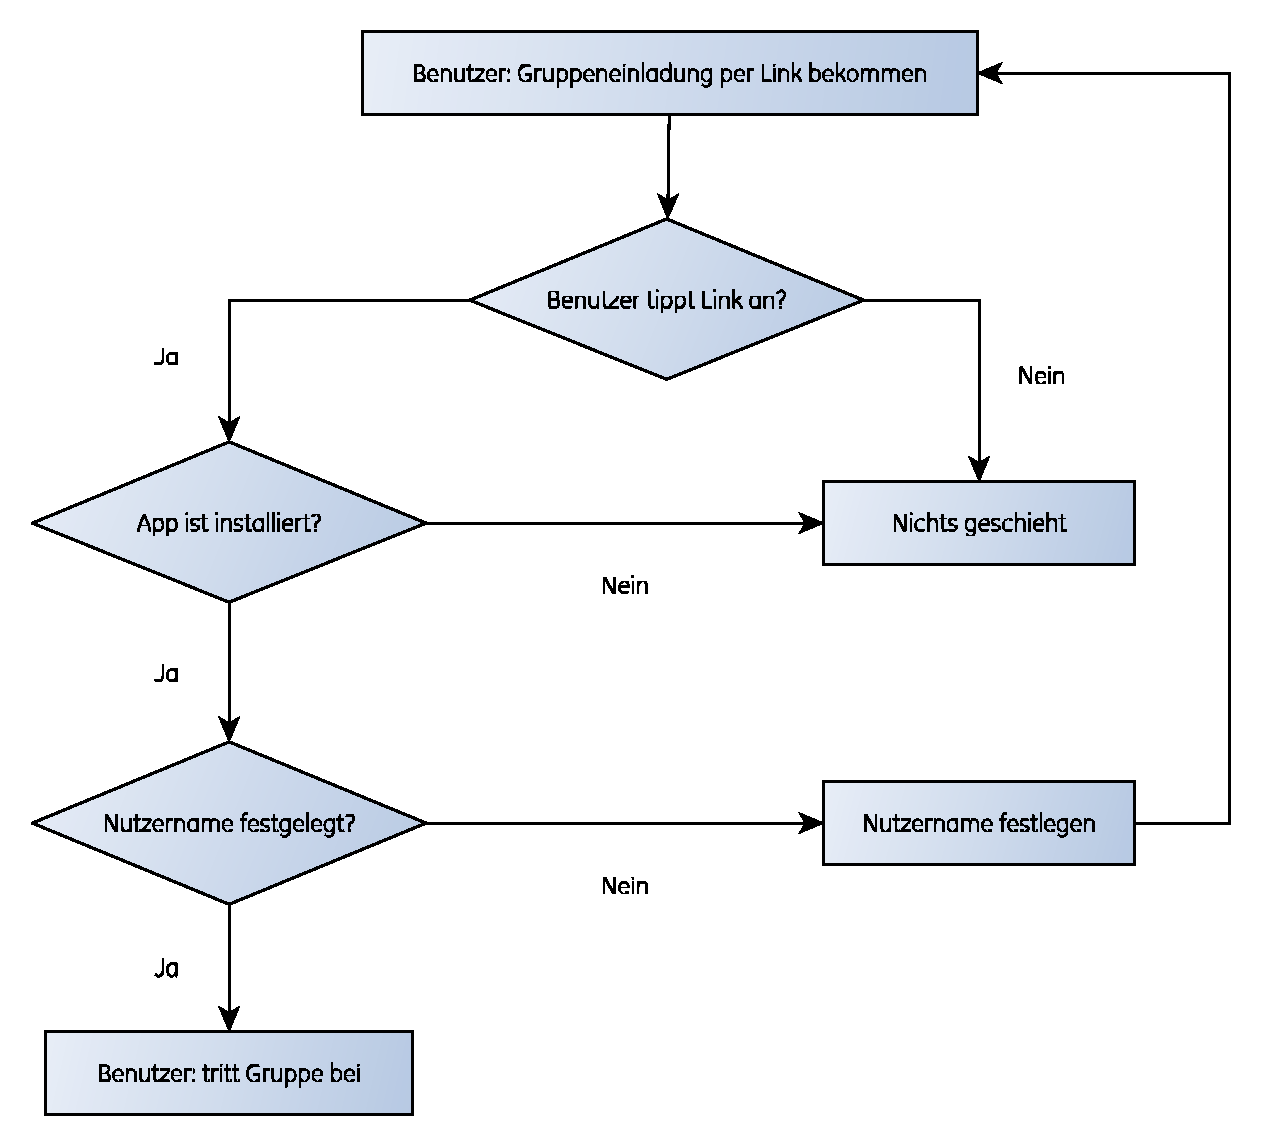
\includegraphics[scale=0.8]{FXX_gruppe_beitreten_flowgraph.pdf}
